\documentclass[tikz,border=8pt]{standalone}
% Shared look for every TikZ diagram. Load with % Shared look for every TikZ diagram. Load with % Shared look for every TikZ diagram. Load with \input{../../tools/tikz-style.tex}
\usepackage[T1]{fontenc}
\usepackage{lmodern}
\renewcommand{\sfdefault}{lmr}  % diagrams use the same serif as the text
\usetikzlibrary{arrows.meta, positioning, shapes.geometric, calc, fit, backgrounds}
\definecolor{cblue}{HTML}{4C78A8}
\definecolor{corange}{HTML}{F58518}
\definecolor{cgreen}{HTML}{54A24B}
\definecolor{cred}{HTML}{E45756}
\definecolor{cpurple}{HTML}{B279A2}
\definecolor{cgrey}{HTML}{6B6B6B}
\tikzset{
  every picture/.style={font=\sffamily, line width=1.2pt},
  box/.style={draw=#1, fill=#1!12, rounded corners=4pt, align=center, inner sep=7pt, minimum height=1.1cm},
  box/.default=cgrey,
  arrow/.style={-{Stealth[length=3mm]}, draw=cgrey, line width=1.4pt},
  title/.style={font=\sffamily\bfseries\Large},
  note/.style={font=\sffamily\small, text=cgrey, align=center},
}
\AtBeginDocument{\hyphenpenalty=10000 \exhyphenpenalty=10000}

\usepackage[T1]{fontenc}
\usepackage{lmodern}
\renewcommand{\sfdefault}{lmr}  % diagrams use the same serif as the text
\usetikzlibrary{arrows.meta, positioning, shapes.geometric, calc, fit, backgrounds}
\definecolor{cblue}{HTML}{4C78A8}
\definecolor{corange}{HTML}{F58518}
\definecolor{cgreen}{HTML}{54A24B}
\definecolor{cred}{HTML}{E45756}
\definecolor{cpurple}{HTML}{B279A2}
\definecolor{cgrey}{HTML}{6B6B6B}
\tikzset{
  every picture/.style={font=\sffamily, line width=1.2pt},
  box/.style={draw=#1, fill=#1!12, rounded corners=4pt, align=center, inner sep=7pt, minimum height=1.1cm},
  box/.default=cgrey,
  arrow/.style={-{Stealth[length=3mm]}, draw=cgrey, line width=1.4pt},
  title/.style={font=\sffamily\bfseries\Large},
  note/.style={font=\sffamily\small, text=cgrey, align=center},
}
\AtBeginDocument{\hyphenpenalty=10000 \exhyphenpenalty=10000}

\usepackage[T1]{fontenc}
\usepackage{lmodern}
\renewcommand{\sfdefault}{lmr}  % diagrams use the same serif as the text
\usetikzlibrary{arrows.meta, positioning, shapes.geometric, calc, fit, backgrounds}
\definecolor{cblue}{HTML}{4C78A8}
\definecolor{corange}{HTML}{F58518}
\definecolor{cgreen}{HTML}{54A24B}
\definecolor{cred}{HTML}{E45756}
\definecolor{cpurple}{HTML}{B279A2}
\definecolor{cgrey}{HTML}{6B6B6B}
\tikzset{
  every picture/.style={font=\sffamily, line width=1.2pt},
  box/.style={draw=#1, fill=#1!12, rounded corners=4pt, align=center, inner sep=7pt, minimum height=1.1cm},
  box/.default=cgrey,
  arrow/.style={-{Stealth[length=3mm]}, draw=cgrey, line width=1.4pt},
  title/.style={font=\sffamily\bfseries\Large},
  note/.style={font=\sffamily\small, text=cgrey, align=center},
}
\AtBeginDocument{\hyphenpenalty=10000 \exhyphenpenalty=10000}

\begin{document}
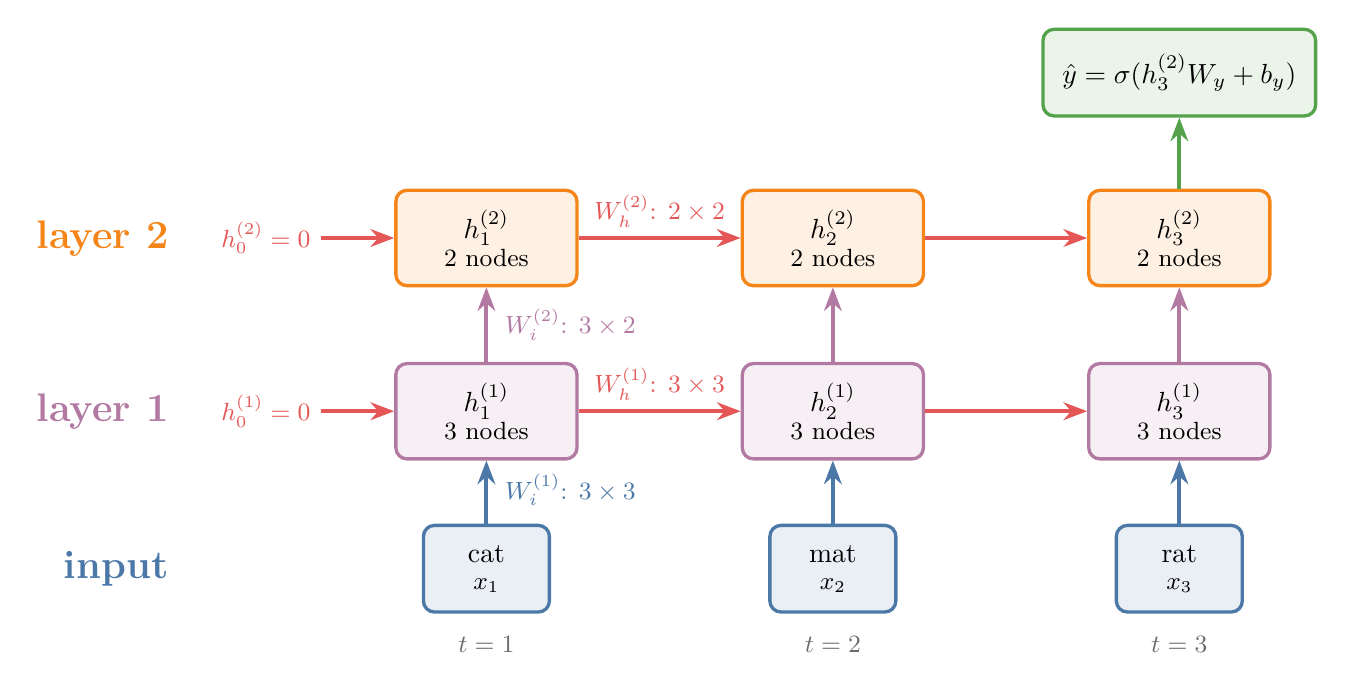
\begin{tikzpicture}[cell/.style={box=#1, minimum width=2.3cm, minimum height=1.0cm}]
  \foreach \t/\w in {1/cat,2/mat,3/rat} {
    \node[box=cblue, minimum width=1.6cm] (x\t) at (4.4*\t,0) {\w\\[-2pt]{\small $x_\t$}};
    \node[cell=cpurple] (a\t) at (4.4*\t,2.0) {$h^{(1)}_\t$\\[-2pt]{\small 3 nodes}};
    \node[cell=corange] (b\t) at (4.4*\t,4.2) {$h^{(2)}_\t$\\[-2pt]{\small 2 nodes}};
    \draw[arrow, draw=cblue] (x\t) -- (a\t);
    \draw[arrow, draw=cpurple] (a\t) -- (b\t);
    \node[note, below=0.15cm of x\t] {$t = \t$};
  }
  \node[note, text=cred] (z1) at (1.6,2.0) {$h^{(1)}_0 = 0$};
  \node[note, text=cred] (z2) at (1.6,4.2) {$h^{(2)}_0 = 0$};
  \draw[arrow, draw=cred] (z1) -- (a1);  \draw[arrow, draw=cred] (z2) -- (b1);
  \draw[arrow, draw=cred] (a1) -- (a2);  \draw[arrow, draw=cred] (a2) -- (a3);
  \draw[arrow, draw=cred] (b1) -- (b2);  \draw[arrow, draw=cred] (b2) -- (b3);
  \node[box=cgreen] (y) at (4.4*3,6.3) {$\hat{y} = \sigma(h^{(2)}_3 W_y + b_y)$};
  \draw[arrow, draw=cgreen] (b3) -- (y);
  % weight labels
  \node[note, text=cblue, anchor=west] at (4.4*1+0.1,1.0) {$W^{(1)}_i$: $3 \times 3$};
  \node[note, text=cpurple, anchor=west] at (4.4*1+0.1,3.1) {$W^{(2)}_i$: $3 \times 2$};
  \node[note, text=cred, above] at (4.4*1.5,2.0) {$W^{(1)}_h$: $3 \times 3$};
  \node[note, text=cred, above] at (4.4*1.5,4.2) {$W^{(2)}_h$: $2 \times 2$};
  \node[title, text=cpurple, anchor=east] at (0.5,2.0) {layer 1};
  \node[title, text=corange, anchor=east] at (0.5,4.2) {layer 2};
  \node[title, text=cblue, anchor=east] at (0.5,0) {input};
\end{tikzpicture}
\end{document}
